\section{Dataset and Method} \label{sec:dataset_and_method}
\subsection{Method} \label{subsec:method}

\begin{figure}[ht]
    \centering
    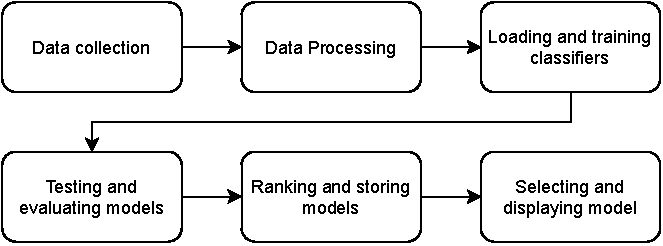
\includegraphics[width=0.7\columnwidth]{media/design/Data_Flow_System.pdf}
    \caption{Training and Selection Process}
    \label{fig:data_flow_in_system}
\end{figure}

The figure \ref{fig:data_flow_in_system}, shows the basic architecture of the automated model training and selection system. The data is collected from the user and processed by the application. This data is stored as training and testing datasets.

\begin{figure}[ht]
    \centering
    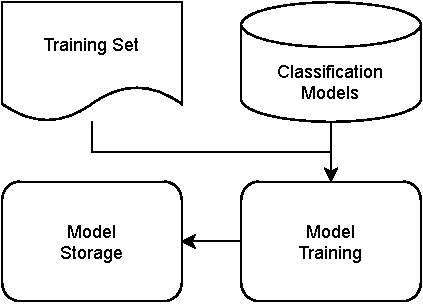
\includegraphics[width=0.7\columnwidth]{media/design/Trainer.pdf}
    \caption{Training Process}
    \label{fig:training_process}
\end{figure}

Figure \ref{fig:training_process}, shows the training process. In this process, the training dataset is loaded into the system. Premade classification model templates are accessed by the system and trained with provided data. These trained models are stored by the system for the next step.

\begin{figure}[ht]
    \centering
    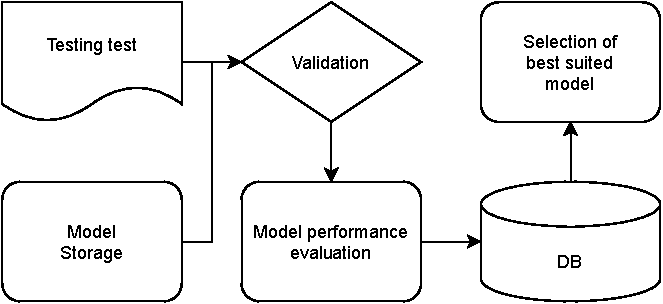
\includegraphics[width=0.7\columnwidth]{media/design/Selector.pdf}
    \caption{Selection Process}
    \label{fig:selection_process}
\end{figure}

The figure \ref{fig:selection_process}, shows the selection process. In this process, the testing dataset is used for the evaluation of the trained models. The trained models are ranked with respect to the performance evaluation. These ranks are used with the help of the tuning parameters to select the best-suited model. This model is stored as the best model for future classification.

\subsection{Dataset}
The ECG readings in this paper are obtained from the MIT-BIH arrhythmia database. This database is used for automated training and evaluation. This dataset was published in 1999 by MIT-BIH as an open-source database; it consists of training and testing datasets. This database is further divided into four equal parts for analysis. Each training set contains 21888 signals, and the testing set contains 5473 signals.